%% GENERATED by scripts/make_figure1.py -- edit the generator, not this file.
\documentclass[border=6pt]{standalone}
\usepackage{tikz}
\usetikzlibrary{arrows.meta}
\usepackage{sansmath}
\renewcommand{\familydefault}{\sfdefault}
\sansmath
\definecolor{ink}{HTML}{1B2430}
\definecolor{inkdim}{HTML}{5D7185}
\definecolor{gridc}{HTML}{C9D3DE}
\definecolor{sph}{HTML}{D9DEE4}
\definecolor{sub}{HTML}{C8CED6}
\definecolor{shellc}{HTML}{EEF1F5}
\definecolor{uhi}{HTML}{1D3A7A}
\definecolor{ulo}{HTML}{F5DFA0}
\definecolor{spA}{HTML}{1D3A7A}
\definecolor{spB}{HTML}{A4C639}
\definecolor{spAB}{HTML}{2BB3A3}
\tikzset{
  gridl/.style={draw=gridc, line width=0.5pt},
  gridb/.style={draw=gridc!70!ink, line width=0.6pt},
  shell/.style={fill=shellc},
  op/.style={-{Stealth[length=7pt,width=5pt]}, line width=1.4pt, ink},
  mv/.style={-{Stealth[length=4pt,width=3.5pt]}, line width=0.9pt, ink},
  gen/.style={-{Stealth[length=5pt]}, line width=0.9pt, inkdim},
  lbl/.style={font=\small, ink},
  reads/.style={-{Stealth[length=5pt]}, line width=0.9pt, inkdim, dashed},
}
\newcommand{\num}[1]{\tikz[baseline=(n.base)]\node[draw=ink, circle, line width=0.6pt, inner sep=0.8pt, font=\scriptsize](n){#1};}
\begin{document}
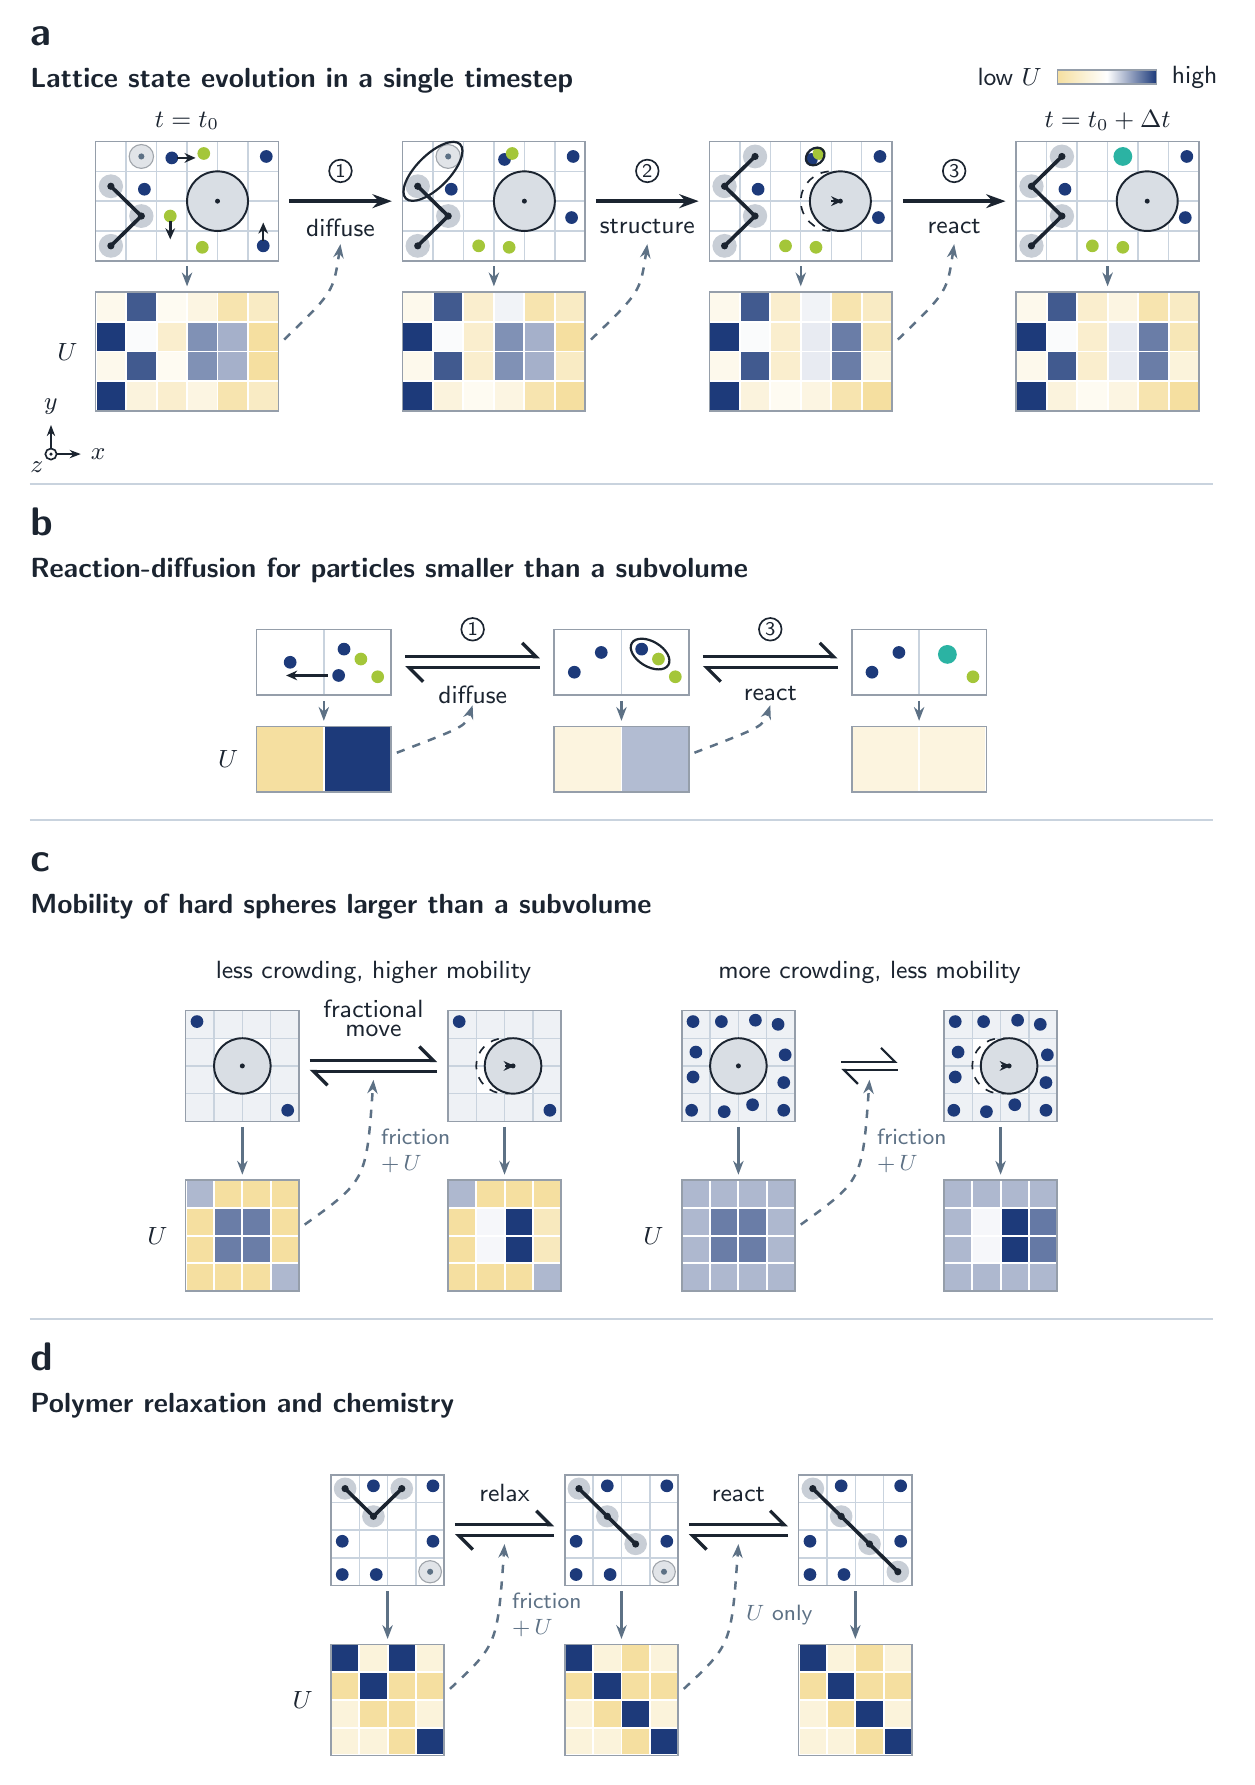
\begin{tikzpicture}[x=0.9cm, y=0.88cm]
\node[anchor=base west, font=\fontsize{14}{16}\selectfont\bfseries, ink, inner sep=0pt] at (-0.100,1.150) {a};
\node[anchor=base west, font=\normalsize\bfseries, ink, inner sep=0pt] at (-0.100,0.550) {Lattice state evolution in a single timestep};
\draw[gridl, shift={(0.830,-1.950)}] (0,0) grid[step=0.430] (2.580,1.720);
\draw[gridb] (0.830,-1.950) rectangle (3.410,-0.230);
\fill[sph, draw=ink, line width=0.7pt] (2.550,-1.090) circle (0.430);
\fill[ink] (2.550,-1.090) circle (0.9pt);
\fill[sub] (1.045,-1.735) circle (0.172);
\fill[sub] (1.475,-1.305) circle (0.172);
\fill[sub] (1.045,-0.875) circle (0.172);
\fill[sub!55!white, draw=sub!80!black, line width=0.4pt] (1.475,-0.445) circle (0.172);
\fill[inkdim] (1.475,-0.445) circle (1.1pt);
\draw[ink, line width=1.3pt] (1.045,-1.735) -- (1.475,-1.305) -- (1.045,-0.875);
\fill[ink] (1.045,-1.735) circle (1.3pt);
\fill[ink] (1.475,-1.305) circle (1.3pt);
\fill[ink] (1.045,-0.875) circle (1.3pt);
\fill[spA] (1.905,-0.466) circle (2.3pt);
\fill[spB] (2.356,-0.402) circle (2.3pt);
\fill[spA] (3.195,-1.735) circle (2.3pt);
\fill[spB] (1.883,-1.305) circle (2.3pt);
\fill[spA] (3.238,-0.445) circle (2.3pt);
\fill[spB] (2.335,-1.756) circle (2.3pt);
\fill[spA] (1.518,-0.918) circle (2.3pt);
\draw[gen] (2.120,-2.030) -- (2.120,-2.320);
\draw[gridl, shift={(5.160,-1.950)}] (0,0) grid[step=0.430] (2.580,1.720);
\draw[gridb] (5.160,-1.950) rectangle (7.740,-0.230);
\fill[sph, draw=ink, line width=0.7pt] (6.880,-1.090) circle (0.430);
\fill[ink] (6.880,-1.090) circle (0.9pt);
\fill[sub] (5.375,-1.735) circle (0.172);
\fill[sub] (5.805,-1.305) circle (0.172);
\fill[sub] (5.375,-0.875) circle (0.172);
\fill[sub!55!white, draw=sub!80!black, line width=0.4pt] (5.805,-0.445) circle (0.172);
\fill[inkdim] (5.805,-0.445) circle (1.1pt);
\draw[ink, line width=1.3pt] (5.375,-1.735) -- (5.805,-1.305) -- (5.375,-0.875);
\fill[ink] (5.375,-1.735) circle (1.3pt);
\fill[ink] (5.805,-1.305) circle (1.3pt);
\fill[ink] (5.375,-0.875) circle (1.3pt);
\fill[spA] (6.600,-0.488) circle (2.3pt);
\fill[spB] (6.708,-0.402) circle (2.3pt);
\fill[spA] (7.546,-1.327) circle (2.3pt);
\fill[spB] (6.235,-1.735) circle (2.3pt);
\fill[spA] (7.568,-0.445) circle (2.3pt);
\fill[spB] (6.665,-1.756) circle (2.3pt);
\fill[spA] (5.848,-0.918) circle (2.3pt);
\draw[gen] (6.450,-2.030) -- (6.450,-2.320);
\draw[gridl, shift={(9.490,-1.950)}] (0,0) grid[step=0.430] (2.580,1.720);
\draw[gridb] (9.490,-1.950) rectangle (12.070,-0.230);
\draw[ink, dashed, line width=0.6pt] (11.210,-1.090) circle (0.430);
\fill[sph, draw=ink, line width=0.7pt] (11.339,-1.090) circle (0.430);
\fill[ink] (11.339,-1.090) circle (0.9pt);
\draw[mv] (11.210,-1.090) -- (11.365,-1.090);
\fill[sub] (9.705,-1.735) circle (0.172);
\fill[sub] (10.135,-1.305) circle (0.172);
\fill[sub] (9.705,-0.875) circle (0.172);
\fill[sub] (10.135,-0.445) circle (0.172);
\draw[ink, line width=1.3pt] (9.705,-1.735) -- (10.135,-1.305) -- (9.705,-0.875) -- (10.135,-0.445);
\fill[ink] (9.705,-1.735) circle (1.3pt);
\fill[ink] (10.135,-1.305) circle (1.3pt);
\fill[ink] (9.705,-0.875) circle (1.3pt);
\fill[ink] (10.135,-0.445) circle (1.3pt);
\fill[spA] (10.930,-0.488) circle (2.3pt);
\fill[spB] (11.038,-0.402) circle (2.3pt);
\fill[spA] (11.876,-1.327) circle (2.3pt);
\fill[spB] (10.565,-1.735) circle (2.3pt);
\fill[spA] (11.898,-0.445) circle (2.3pt);
\fill[spB] (10.995,-1.756) circle (2.3pt);
\fill[spA] (10.178,-0.918) circle (2.3pt);
\draw[gen] (10.780,-2.030) -- (10.780,-2.320);
\draw[gridl, shift={(13.820,-1.950)}] (0,0) grid[step=0.430] (2.580,1.720);
\draw[gridb] (13.820,-1.950) rectangle (16.400,-0.230);
\fill[sph, draw=ink, line width=0.7pt] (15.669,-1.090) circle (0.430);
\fill[ink] (15.669,-1.090) circle (0.9pt);
\fill[sub] (14.035,-1.735) circle (0.172);
\fill[sub] (14.465,-1.305) circle (0.172);
\fill[sub] (14.035,-0.875) circle (0.172);
\fill[sub] (14.465,-0.445) circle (0.172);
\draw[ink, line width=1.3pt] (14.035,-1.735) -- (14.465,-1.305) -- (14.035,-0.875) -- (14.465,-0.445);
\fill[ink] (14.035,-1.735) circle (1.3pt);
\fill[ink] (14.465,-1.305) circle (1.3pt);
\fill[ink] (14.035,-0.875) circle (1.3pt);
\fill[ink] (14.465,-0.445) circle (1.3pt);
\fill[spAB] (15.325,-0.445) circle (3.4pt);
\fill[spA] (16.206,-1.327) circle (2.3pt);
\fill[spB] (14.895,-1.735) circle (2.3pt);
\fill[spA] (16.228,-0.445) circle (2.3pt);
\fill[spB] (15.325,-1.756) circle (2.3pt);
\fill[spA] (14.508,-0.918) circle (2.3pt);
\draw[gen] (15.110,-2.030) -- (15.110,-2.320);
\draw[mv] (1.974,-0.466) -- ++(0.267,0.000);
\draw[mv] (3.195,-1.666) -- ++(0.000,0.267);
\draw[mv] (1.883,-1.374) -- ++(0.000,-0.267);
\draw[ink, line width=0.8pt, rotate around={38.7:(10.984,-0.445)}] (10.984,-0.445) ellipse (0.142 and 0.115);
\draw[ink, line width=0.8pt, rotate around={45.0:(5.590,-0.660)}] (5.590,-0.660) ellipse (0.541 and 0.237);
\draw[op] (3.560,-1.090) -- (5.010,-1.090);
\node[lbl, above=3pt] at (4.285,-1.090) {\num{1}};
\node[lbl, below=3pt] at (4.285,-1.090) {diffuse};
\draw[op] (7.890,-1.090) -- (9.340,-1.090);
\node[lbl, above=3pt] at (8.615,-1.090) {\num{2}};
\node[lbl, below=3pt] at (8.615,-1.090) {structure};
\draw[op] (12.220,-1.090) -- (13.670,-1.090);
\node[lbl, above=3pt] at (12.945,-1.090) {\num{3}};
\node[lbl, below=3pt] at (12.945,-1.090) {react};
\node[lbl, anchor=center] at (2.120,0.070) {$t=t_0$};
\node[lbl, anchor=center] at (15.110,0.070) {$t=t_0+\Delta t$};
\draw[reads] (3.490,-3.088) .. controls (4.185,-2.400) .. (4.285,-1.710);
\draw[reads] (7.820,-3.088) .. controls (8.515,-2.400) .. (8.615,-1.710);
\draw[reads] (12.150,-3.088) .. controls (12.845,-2.400) .. (12.945,-1.710);
\node[lbl, anchor=east] at (0.710,-3.260) {$U$};
\draw[-{Stealth[length=4pt]}, line width=0.7pt, ink] (0.200,-4.740) -- ++(0.420,0) node[right=0pt, font=\small] {$x$};
\draw[-{Stealth[length=4pt]}, line width=0.7pt, ink] (0.200,-4.740) -- ++(0,0.420) node[above=0pt, font=\small] {$y$};
\draw[ink, line width=0.6pt, fill=white] (0.200,-4.740) circle (0.08);
\fill[ink] (0.200,-4.740) circle (0.025);
\node[font=\small, ink, anchor=north east, inner sep=1pt] at (0.140,-4.800) {$z$};
\shade[left color=ulo, right color=uhi, middle color=white, draw=gridc!70!ink, line width=0.5pt] (14.400,0.600) rectangle ++(1.4,0.2);
\node[lbl, anchor=east] at (14.320,0.700) {low $U$};
\node[lbl, anchor=west] at (15.880,0.700) {high};
\fill[uhi!100!white] (0.830,-4.120) rectangle ++(0.430,0.430);
\fill[ulo!36!white] (1.260,-4.120) rectangle ++(0.430,0.430);
\fill[ulo!52!white] (1.690,-4.120) rectangle ++(0.430,0.430);
\fill[ulo!30!white] (2.120,-4.120) rectangle ++(0.430,0.430);
\fill[ulo!84!white] (2.550,-4.120) rectangle ++(0.430,0.430);
\fill[ulo!62!white] (2.980,-4.120) rectangle ++(0.430,0.430);
\fill[ulo!20!white] (0.830,-3.690) rectangle ++(0.430,0.430);
\fill[uhi!84!white] (1.260,-3.690) rectangle ++(0.430,0.430);
\fill[ulo!14!white] (1.690,-3.690) rectangle ++(0.430,0.430);
\fill[uhi!56!white] (2.120,-3.690) rectangle ++(0.430,0.430);
\fill[uhi!40!white] (2.550,-3.690) rectangle ++(0.430,0.430);
\fill[ulo!100!white] (2.980,-3.690) rectangle ++(0.430,0.430);
\fill[uhi!100!white] (0.830,-3.260) rectangle ++(0.430,0.430);
\fill[uhi!2!white] (1.260,-3.260) rectangle ++(0.430,0.430);
\fill[ulo!52!white] (1.690,-3.260) rectangle ++(0.430,0.430);
\fill[uhi!56!white] (2.120,-3.260) rectangle ++(0.430,0.430);
\fill[uhi!40!white] (2.550,-3.260) rectangle ++(0.430,0.430);
\fill[ulo!100!white] (2.980,-3.260) rectangle ++(0.430,0.430);
\fill[ulo!20!white] (0.830,-2.830) rectangle ++(0.430,0.430);
\fill[uhi!84!white] (1.260,-2.830) rectangle ++(0.430,0.430);
\fill[ulo!14!white] (1.690,-2.830) rectangle ++(0.430,0.430);
\fill[ulo!30!white] (2.120,-2.830) rectangle ++(0.430,0.430);
\fill[ulo!84!white] (2.550,-2.830) rectangle ++(0.430,0.430);
\fill[ulo!62!white] (2.980,-2.830) rectangle ++(0.430,0.430);
\draw[white, line width=0.7pt, shift={(0.830,-4.120)}] (0,0) grid[step=0.430] (2.580,1.720);
\draw[gridb] (0.830,-4.120) rectangle (3.410,-2.400);
\fill[uhi!100!white] (5.160,-4.120) rectangle ++(0.430,0.430);
\fill[ulo!36!white] (5.590,-4.120) rectangle ++(0.430,0.430);
\fill[ulo!14!white] (6.020,-4.120) rectangle ++(0.430,0.430);
\fill[ulo!30!white] (6.450,-4.120) rectangle ++(0.430,0.430);
\fill[ulo!84!white] (6.880,-4.120) rectangle ++(0.430,0.430);
\fill[ulo!100!white] (7.310,-4.120) rectangle ++(0.430,0.430);
\fill[ulo!20!white] (5.160,-3.690) rectangle ++(0.430,0.430);
\fill[uhi!84!white] (5.590,-3.690) rectangle ++(0.430,0.430);
\fill[ulo!52!white] (6.020,-3.690) rectangle ++(0.430,0.430);
\fill[uhi!56!white] (6.450,-3.690) rectangle ++(0.430,0.430);
\fill[uhi!40!white] (6.880,-3.690) rectangle ++(0.430,0.430);
\fill[ulo!62!white] (7.310,-3.690) rectangle ++(0.430,0.430);
\fill[uhi!100!white] (5.160,-3.260) rectangle ++(0.430,0.430);
\fill[uhi!2!white] (5.590,-3.260) rectangle ++(0.430,0.430);
\fill[ulo!52!white] (6.020,-3.260) rectangle ++(0.430,0.430);
\fill[uhi!56!white] (6.450,-3.260) rectangle ++(0.430,0.430);
\fill[uhi!40!white] (6.880,-3.260) rectangle ++(0.430,0.430);
\fill[ulo!100!white] (7.310,-3.260) rectangle ++(0.430,0.430);
\fill[ulo!20!white] (5.160,-2.830) rectangle ++(0.430,0.430);
\fill[uhi!84!white] (5.590,-2.830) rectangle ++(0.430,0.430);
\fill[ulo!52!white] (6.020,-2.830) rectangle ++(0.430,0.430);
\fill[uhi!6!white] (6.450,-2.830) rectangle ++(0.430,0.430);
\fill[ulo!84!white] (6.880,-2.830) rectangle ++(0.430,0.430);
\fill[ulo!62!white] (7.310,-2.830) rectangle ++(0.430,0.430);
\draw[white, line width=0.7pt, shift={(5.160,-4.120)}] (0,0) grid[step=0.430] (2.580,1.720);
\draw[gridb] (5.160,-4.120) rectangle (7.740,-2.400);
\fill[uhi!100!white] (9.490,-4.120) rectangle ++(0.430,0.430);
\fill[ulo!36!white] (9.920,-4.120) rectangle ++(0.430,0.430);
\fill[ulo!14!white] (10.350,-4.120) rectangle ++(0.430,0.430);
\fill[ulo!30!white] (10.780,-4.120) rectangle ++(0.430,0.430);
\fill[ulo!84!white] (11.210,-4.120) rectangle ++(0.430,0.430);
\fill[ulo!100!white] (11.640,-4.120) rectangle ++(0.430,0.430);
\fill[ulo!20!white] (9.490,-3.690) rectangle ++(0.430,0.430);
\fill[uhi!84!white] (9.920,-3.690) rectangle ++(0.430,0.430);
\fill[ulo!52!white] (10.350,-3.690) rectangle ++(0.430,0.430);
\fill[uhi!10!white] (10.780,-3.690) rectangle ++(0.430,0.430);
\fill[uhi!66!white] (11.210,-3.690) rectangle ++(0.430,0.430);
\fill[ulo!38!white] (11.640,-3.690) rectangle ++(0.430,0.430);
\fill[uhi!100!white] (9.490,-3.260) rectangle ++(0.430,0.430);
\fill[uhi!2!white] (9.920,-3.260) rectangle ++(0.430,0.430);
\fill[ulo!52!white] (10.350,-3.260) rectangle ++(0.430,0.430);
\fill[uhi!10!white] (10.780,-3.260) rectangle ++(0.430,0.430);
\fill[uhi!66!white] (11.210,-3.260) rectangle ++(0.430,0.430);
\fill[ulo!76!white] (11.640,-3.260) rectangle ++(0.430,0.430);
\fill[ulo!20!white] (9.490,-2.830) rectangle ++(0.430,0.430);
\fill[uhi!84!white] (9.920,-2.830) rectangle ++(0.430,0.430);
\fill[ulo!52!white] (10.350,-2.830) rectangle ++(0.430,0.430);
\fill[uhi!6!white] (10.780,-2.830) rectangle ++(0.430,0.430);
\fill[ulo!84!white] (11.210,-2.830) rectangle ++(0.430,0.430);
\fill[ulo!62!white] (11.640,-2.830) rectangle ++(0.430,0.430);
\draw[white, line width=0.7pt, shift={(9.490,-4.120)}] (0,0) grid[step=0.430] (2.580,1.720);
\draw[gridb] (9.490,-4.120) rectangle (12.070,-2.400);
\fill[uhi!100!white] (13.820,-4.120) rectangle ++(0.430,0.430);
\fill[ulo!36!white] (14.250,-4.120) rectangle ++(0.430,0.430);
\fill[ulo!14!white] (14.680,-4.120) rectangle ++(0.430,0.430);
\fill[ulo!30!white] (15.110,-4.120) rectangle ++(0.430,0.430);
\fill[ulo!84!white] (15.540,-4.120) rectangle ++(0.430,0.430);
\fill[ulo!100!white] (15.970,-4.120) rectangle ++(0.430,0.430);
\fill[ulo!20!white] (13.820,-3.690) rectangle ++(0.430,0.430);
\fill[uhi!84!white] (14.250,-3.690) rectangle ++(0.430,0.430);
\fill[ulo!52!white] (14.680,-3.690) rectangle ++(0.430,0.430);
\fill[uhi!10!white] (15.110,-3.690) rectangle ++(0.430,0.430);
\fill[uhi!66!white] (15.540,-3.690) rectangle ++(0.430,0.430);
\fill[ulo!38!white] (15.970,-3.690) rectangle ++(0.430,0.430);
\fill[uhi!100!white] (13.820,-3.260) rectangle ++(0.430,0.430);
\fill[uhi!2!white] (14.250,-3.260) rectangle ++(0.430,0.430);
\fill[ulo!52!white] (14.680,-3.260) rectangle ++(0.430,0.430);
\fill[uhi!10!white] (15.110,-3.260) rectangle ++(0.430,0.430);
\fill[uhi!66!white] (15.540,-3.260) rectangle ++(0.430,0.430);
\fill[ulo!76!white] (15.970,-3.260) rectangle ++(0.430,0.430);
\fill[ulo!20!white] (13.820,-2.830) rectangle ++(0.430,0.430);
\fill[uhi!84!white] (14.250,-2.830) rectangle ++(0.430,0.430);
\fill[ulo!52!white] (14.680,-2.830) rectangle ++(0.430,0.430);
\fill[ulo!30!white] (15.110,-2.830) rectangle ++(0.430,0.430);
\fill[ulo!84!white] (15.540,-2.830) rectangle ++(0.430,0.430);
\fill[ulo!62!white] (15.970,-2.830) rectangle ++(0.430,0.430);
\draw[white, line width=0.7pt, shift={(13.820,-4.120)}] (0,0) grid[step=0.430] (2.580,1.720);
\draw[gridb] (13.820,-4.120) rectangle (16.400,-2.400);
\draw[gridc, line width=0.6pt] (-0.1,-5.170) -- (16.6,-5.170);
\node[anchor=base west, font=\fontsize{14}{16}\selectfont\bfseries, ink, inner sep=0pt] at (-0.100,-5.920) {b};
\node[anchor=base west, font=\normalsize\bfseries, ink, inner sep=0pt] at (-0.100,-6.520) {Reaction-diffusion for particles smaller than a subvolume};
\draw[gridl, shift={(3.100,-8.220)}] (0,0) grid[step=0.950] (1.900,0.950);
\draw[gridb] (3.100,-8.220) rectangle (5.000,-7.270);
\fill[spA] (3.575,-7.745) circle (2.3pt);
\fill[spA] (4.259,-7.935) circle (2.3pt);
\fill[spA] (4.335,-7.555) circle (2.3pt);
\fill[spB] (4.573,-7.698) circle (2.3pt);
\fill[spB] (4.810,-7.954) circle (2.3pt);
\draw[gen] (4.050,-8.300) -- (4.050,-8.590);
\draw[gridl, shift={(7.300,-8.220)}] (0,0) grid[step=0.950] (1.900,0.950);
\draw[gridb] (7.300,-8.220) rectangle (9.200,-7.270);
\fill[spA] (7.585,-7.888) circle (2.3pt);
\fill[spA] (7.965,-7.603) circle (2.3pt);
\fill[spA] (8.535,-7.555) circle (2.3pt);
\fill[spB] (8.772,-7.698) circle (2.3pt);
\fill[spB] (9.010,-7.954) circle (2.3pt);
\draw[gen] (8.250,-8.300) -- (8.250,-8.590);
\draw[gridl, shift={(11.500,-8.220)}] (0,0) grid[step=0.950] (1.900,0.950);
\draw[gridb] (11.500,-8.220) rectangle (13.400,-7.270);
\fill[spA] (11.785,-7.888) circle (2.3pt);
\fill[spA] (12.165,-7.603) circle (2.3pt);
\fill[spAB] (12.849,-7.631) circle (3.4pt);
\fill[spB] (13.210,-7.954) circle (2.3pt);
\draw[gen] (12.450,-8.300) -- (12.450,-8.590);
\draw[mv] (4.107,-7.935) -- ++(-0.589,0.000);
\draw[ink, line width=0.8pt, rotate around={-31.0:(8.654,-7.626)}] (8.654,-7.626) ellipse (0.300 and 0.181);
\draw[-{Straight Barb[left,length=5pt]}, line width=1.2pt, ink] (5.200,-7.665) -- (7.100,-7.665);
\draw[-{Straight Barb[left,length=5pt]}, line width=1.2pt, ink] (7.100,-7.825) -- (5.200,-7.825);
\node[lbl, above=4pt] at (6.150,-7.745) {\num{1}};
\node[lbl, below=5pt] at (6.150,-7.745) {diffuse};
\draw[-{Straight Barb[left,length=5pt]}, line width=1.2pt, ink] (9.400,-7.665) -- (11.300,-7.665);
\draw[-{Straight Barb[left,length=5pt]}, line width=1.2pt, ink] (11.300,-7.825) -- (9.400,-7.825);
\node[lbl, above=4pt] at (10.350,-7.745) {\num{3}};
\node[lbl, below=5pt] at (10.350,-7.745) {react};
\draw[reads] (5.080,-9.050) .. controls (6.050,-8.670) .. (6.150,-8.365);
\draw[reads] (9.280,-9.050) .. controls (10.250,-8.670) .. (10.350,-8.365);
\node[lbl, anchor=east] at (2.980,-9.145) {$U$};
\fill[ulo!100!white] (3.100,-9.620) rectangle ++(0.950,0.950);
\fill[uhi!100!white] (4.050,-9.620) rectangle ++(0.950,0.950);
\draw[white, line width=0.7pt, shift={(3.100,-9.620)}] (0,0) grid[step=0.950] (1.900,0.950);
\draw[gridb] (3.100,-9.620) rectangle (5.000,-8.670);
\fill[ulo!34!white] (7.300,-9.620) rectangle ++(0.950,0.950);
\fill[uhi!34!white] (8.250,-9.620) rectangle ++(0.950,0.950);
\draw[white, line width=0.7pt, shift={(7.300,-9.620)}] (0,0) grid[step=0.950] (1.900,0.950);
\draw[gridb] (7.300,-9.620) rectangle (9.200,-8.670);
\fill[ulo!34!white] (11.500,-9.620) rectangle ++(0.950,0.950);
\fill[ulo!34!white] (12.450,-9.620) rectangle ++(0.950,0.950);
\draw[white, line width=0.7pt, shift={(11.500,-9.620)}] (0,0) grid[step=0.950] (1.900,0.950);
\draw[gridb] (11.500,-9.620) rectangle (13.400,-8.670);
\draw[gridc, line width=0.6pt] (-0.1,-10.020) -- (16.6,-10.020);
\node[anchor=base west, font=\fontsize{14}{16}\selectfont\bfseries, ink, inner sep=0pt] at (-0.100,-10.770) {c};
\node[anchor=base west, font=\normalsize\bfseries, ink, inner sep=0pt] at (-0.100,-11.370) {Mobility of hard spheres larger than a subvolume};
\fill[shell] (2.100,-14.370) rectangle ++(0.400,0.400);
\fill[shell] (2.100,-13.970) rectangle ++(0.400,0.400);
\fill[shell] (2.100,-13.570) rectangle ++(0.400,0.400);
\fill[shell] (2.100,-13.170) rectangle ++(0.400,0.400);
\fill[shell] (2.500,-14.370) rectangle ++(0.400,0.400);
\fill[shell] (2.500,-13.170) rectangle ++(0.400,0.400);
\fill[shell] (2.900,-14.370) rectangle ++(0.400,0.400);
\fill[shell] (2.900,-13.170) rectangle ++(0.400,0.400);
\fill[shell] (3.300,-14.370) rectangle ++(0.400,0.400);
\fill[shell] (3.300,-13.970) rectangle ++(0.400,0.400);
\fill[shell] (3.300,-13.570) rectangle ++(0.400,0.400);
\fill[shell] (3.300,-13.170) rectangle ++(0.400,0.400);
\draw[gridl, shift={(2.100,-14.370)}] (0,0) grid[step=0.400] (1.600,1.600);
\draw[gridb] (2.100,-14.370) rectangle (3.700,-12.770);
\fill[sph, draw=ink, line width=0.7pt] (2.900,-13.570) circle (0.400);
\fill[ink] (2.900,-13.570) circle (0.9pt);
\fill[spA] (2.260,-12.930) circle (2.3pt);
\fill[spA] (3.540,-14.210) circle (2.3pt);
\draw[gen] (2.900,-14.450) -- (2.900,-15.140);
\fill[shell] (5.800,-14.370) rectangle ++(0.400,0.400);
\fill[shell] (5.800,-13.970) rectangle ++(0.400,0.400);
\fill[shell] (5.800,-13.570) rectangle ++(0.400,0.400);
\fill[shell] (5.800,-13.170) rectangle ++(0.400,0.400);
\fill[shell] (6.200,-14.370) rectangle ++(0.400,0.400);
\fill[shell] (6.200,-13.170) rectangle ++(0.400,0.400);
\fill[shell] (6.600,-14.370) rectangle ++(0.400,0.400);
\fill[shell] (6.600,-13.170) rectangle ++(0.400,0.400);
\fill[shell] (7.000,-14.370) rectangle ++(0.400,0.400);
\fill[shell] (7.000,-13.970) rectangle ++(0.400,0.400);
\fill[shell] (7.000,-13.570) rectangle ++(0.400,0.400);
\fill[shell] (7.000,-13.170) rectangle ++(0.400,0.400);
\draw[gridl, shift={(5.800,-14.370)}] (0,0) grid[step=0.400] (1.600,1.600);
\draw[gridb] (5.800,-14.370) rectangle (7.400,-12.770);
\draw[ink, dashed, line width=0.6pt] (6.600,-13.570) circle (0.400);
\fill[sph, draw=ink, line width=0.7pt] (6.720,-13.570) circle (0.400);
\fill[ink] (6.720,-13.570) circle (0.9pt);
\draw[mv] (6.600,-13.570) -- (6.744,-13.570);
\fill[spA] (5.960,-12.930) circle (2.3pt);
\fill[spA] (7.240,-14.210) circle (2.3pt);
\draw[gen] (6.600,-14.450) -- (6.600,-15.140);
\draw[-{Straight Barb[left,length=5pt]}, line width=1.2pt, ink] (3.850,-13.490) -- (5.650,-13.490);
\draw[-{Straight Barb[left,length=5pt]}, line width=1.2pt, ink] (5.650,-13.650) -- (3.850,-13.650);
\node[lbl, above=7pt] at (4.750,-13.570) {\shortstack{fractional\\move}};
\draw[reads] (3.780,-15.860) .. controls (4.650,-15.220) .. (4.750,-13.770);
\node[anchor=west, align=left, font=\footnotesize, inkdim, inner sep=0pt] at (4.850,-14.795) {friction\\$+\,U$};
\node[lbl, anchor=center] at (4.750,-12.220) {less crowding, higher mobility};
\node[lbl, anchor=east] at (1.980,-16.020) {$U$};
\fill[shell] (9.100,-14.370) rectangle ++(0.400,0.400);
\fill[shell] (9.100,-13.970) rectangle ++(0.400,0.400);
\fill[shell] (9.100,-13.570) rectangle ++(0.400,0.400);
\fill[shell] (9.100,-13.170) rectangle ++(0.400,0.400);
\fill[shell] (9.500,-14.370) rectangle ++(0.400,0.400);
\fill[shell] (9.500,-13.170) rectangle ++(0.400,0.400);
\fill[shell] (9.900,-14.370) rectangle ++(0.400,0.400);
\fill[shell] (9.900,-13.170) rectangle ++(0.400,0.400);
\fill[shell] (10.300,-14.370) rectangle ++(0.400,0.400);
\fill[shell] (10.300,-13.970) rectangle ++(0.400,0.400);
\fill[shell] (10.300,-13.570) rectangle ++(0.400,0.400);
\fill[shell] (10.300,-13.170) rectangle ++(0.400,0.400);
\draw[gridl, shift={(9.100,-14.370)}] (0,0) grid[step=0.400] (1.600,1.600);
\draw[gridb] (9.100,-14.370) rectangle (10.700,-12.770);
\fill[sph, draw=ink, line width=0.7pt] (9.900,-13.570) circle (0.400);
\fill[ink] (9.900,-13.570) circle (0.9pt);
\fill[spA] (9.260,-12.930) circle (2.3pt);
\fill[spA] (10.540,-14.210) circle (2.3pt);
\fill[spA] (9.240,-14.210) circle (2.3pt);
\fill[spA] (9.260,-13.730) circle (2.3pt);
\fill[spA] (9.700,-14.230) circle (2.3pt);
\fill[spA] (10.140,-12.910) circle (2.3pt);
\fill[spA] (10.560,-13.410) circle (2.3pt);
\fill[spA] (10.540,-13.810) circle (2.3pt);
\fill[spA] (9.660,-12.930) circle (2.3pt);
\fill[spA] (9.300,-13.370) circle (2.3pt);
\fill[spA] (10.100,-14.130) circle (2.3pt);
\fill[spA] (10.460,-12.970) circle (2.3pt);
\draw[gen] (9.900,-14.450) -- (9.900,-15.140);
\fill[shell] (12.800,-14.370) rectangle ++(0.400,0.400);
\fill[shell] (12.800,-13.970) rectangle ++(0.400,0.400);
\fill[shell] (12.800,-13.570) rectangle ++(0.400,0.400);
\fill[shell] (12.800,-13.170) rectangle ++(0.400,0.400);
\fill[shell] (13.200,-14.370) rectangle ++(0.400,0.400);
\fill[shell] (13.200,-13.170) rectangle ++(0.400,0.400);
\fill[shell] (13.600,-14.370) rectangle ++(0.400,0.400);
\fill[shell] (13.600,-13.170) rectangle ++(0.400,0.400);
\fill[shell] (14.000,-14.370) rectangle ++(0.400,0.400);
\fill[shell] (14.000,-13.970) rectangle ++(0.400,0.400);
\fill[shell] (14.000,-13.570) rectangle ++(0.400,0.400);
\fill[shell] (14.000,-13.170) rectangle ++(0.400,0.400);
\draw[gridl, shift={(12.800,-14.370)}] (0,0) grid[step=0.400] (1.600,1.600);
\draw[gridb] (12.800,-14.370) rectangle (14.400,-12.770);
\draw[ink, dashed, line width=0.6pt] (13.600,-13.570) circle (0.400);
\fill[sph, draw=ink, line width=0.7pt] (13.720,-13.570) circle (0.400);
\fill[ink] (13.720,-13.570) circle (0.9pt);
\draw[mv] (13.600,-13.570) -- (13.744,-13.570);
\fill[spA] (12.960,-12.930) circle (2.3pt);
\fill[spA] (14.240,-14.210) circle (2.3pt);
\fill[spA] (12.940,-14.210) circle (2.3pt);
\fill[spA] (12.960,-13.730) circle (2.3pt);
\fill[spA] (13.400,-14.230) circle (2.3pt);
\fill[spA] (13.840,-12.910) circle (2.3pt);
\fill[spA] (14.260,-13.410) circle (2.3pt);
\fill[spA] (14.240,-13.810) circle (2.3pt);
\fill[spA] (13.360,-12.930) circle (2.3pt);
\fill[spA] (13.000,-13.370) circle (2.3pt);
\fill[spA] (13.800,-14.130) circle (2.3pt);
\fill[spA] (14.160,-12.970) circle (2.3pt);
\draw[gen] (13.600,-14.450) -- (13.600,-15.140);
\draw[-{Straight Barb[left,length=5pt]}, line width=0.8pt, ink] (11.354,-13.510) -- (12.146,-13.510);
\draw[-{Straight Barb[left,length=5pt]}, line width=0.8pt, ink] (12.146,-13.630) -- (11.354,-13.630);
\draw[reads] (10.780,-15.860) .. controls (11.650,-15.220) .. (11.750,-13.770);
\node[anchor=west, align=left, font=\footnotesize, inkdim, inner sep=0pt] at (11.850,-14.795) {friction\\$+\,U$};
\node[lbl, anchor=center] at (11.750,-12.220) {more crowding, less mobility};
\node[lbl, anchor=east] at (8.980,-16.020) {$U$};
\fill[ulo!100!white] (2.100,-16.820) rectangle ++(0.400,0.400);
\fill[ulo!100!white] (2.500,-16.820) rectangle ++(0.400,0.400);
\fill[ulo!100!white] (2.900,-16.820) rectangle ++(0.400,0.400);
\fill[uhi!36!white] (3.300,-16.820) rectangle ++(0.400,0.400);
\fill[ulo!100!white] (2.100,-16.420) rectangle ++(0.400,0.400);
\fill[uhi!66!white] (2.500,-16.420) rectangle ++(0.400,0.400);
\fill[uhi!66!white] (2.900,-16.420) rectangle ++(0.400,0.400);
\fill[ulo!100!white] (3.300,-16.420) rectangle ++(0.400,0.400);
\fill[ulo!100!white] (2.100,-16.020) rectangle ++(0.400,0.400);
\fill[uhi!66!white] (2.500,-16.020) rectangle ++(0.400,0.400);
\fill[uhi!66!white] (2.900,-16.020) rectangle ++(0.400,0.400);
\fill[ulo!100!white] (3.300,-16.020) rectangle ++(0.400,0.400);
\fill[uhi!36!white] (2.100,-15.620) rectangle ++(0.400,0.400);
\fill[ulo!100!white] (2.500,-15.620) rectangle ++(0.400,0.400);
\fill[ulo!100!white] (2.900,-15.620) rectangle ++(0.400,0.400);
\fill[ulo!100!white] (3.300,-15.620) rectangle ++(0.400,0.400);
\draw[white, line width=0.7pt, shift={(2.100,-16.820)}] (0,0) grid[step=0.400] (1.600,1.600);
\draw[gridb] (2.100,-16.820) rectangle (3.700,-15.220);
\fill[ulo!100!white] (5.800,-16.820) rectangle ++(0.400,0.400);
\fill[ulo!100!white] (6.200,-16.820) rectangle ++(0.400,0.400);
\fill[ulo!100!white] (6.600,-16.820) rectangle ++(0.400,0.400);
\fill[uhi!36!white] (7.000,-16.820) rectangle ++(0.400,0.400);
\fill[ulo!100!white] (5.800,-16.420) rectangle ++(0.400,0.400);
\fill[uhi!4!white] (6.200,-16.420) rectangle ++(0.400,0.400);
\fill[uhi!100!white] (6.600,-16.420) rectangle ++(0.400,0.400);
\fill[ulo!68!white] (7.000,-16.420) rectangle ++(0.400,0.400);
\fill[ulo!100!white] (5.800,-16.020) rectangle ++(0.400,0.400);
\fill[uhi!4!white] (6.200,-16.020) rectangle ++(0.400,0.400);
\fill[uhi!100!white] (6.600,-16.020) rectangle ++(0.400,0.400);
\fill[ulo!68!white] (7.000,-16.020) rectangle ++(0.400,0.400);
\fill[uhi!36!white] (5.800,-15.620) rectangle ++(0.400,0.400);
\fill[ulo!100!white] (6.200,-15.620) rectangle ++(0.400,0.400);
\fill[ulo!100!white] (6.600,-15.620) rectangle ++(0.400,0.400);
\fill[ulo!100!white] (7.000,-15.620) rectangle ++(0.400,0.400);
\draw[white, line width=0.7pt, shift={(5.800,-16.820)}] (0,0) grid[step=0.400] (1.600,1.600);
\draw[gridb] (5.800,-16.820) rectangle (7.400,-15.220);
\fill[uhi!36!white] (9.100,-16.820) rectangle ++(0.400,0.400);
\fill[uhi!36!white] (9.500,-16.820) rectangle ++(0.400,0.400);
\fill[uhi!36!white] (9.900,-16.820) rectangle ++(0.400,0.400);
\fill[uhi!36!white] (10.300,-16.820) rectangle ++(0.400,0.400);
\fill[uhi!36!white] (9.100,-16.420) rectangle ++(0.400,0.400);
\fill[uhi!66!white] (9.500,-16.420) rectangle ++(0.400,0.400);
\fill[uhi!66!white] (9.900,-16.420) rectangle ++(0.400,0.400);
\fill[uhi!36!white] (10.300,-16.420) rectangle ++(0.400,0.400);
\fill[uhi!36!white] (9.100,-16.020) rectangle ++(0.400,0.400);
\fill[uhi!66!white] (9.500,-16.020) rectangle ++(0.400,0.400);
\fill[uhi!66!white] (9.900,-16.020) rectangle ++(0.400,0.400);
\fill[uhi!36!white] (10.300,-16.020) rectangle ++(0.400,0.400);
\fill[uhi!36!white] (9.100,-15.620) rectangle ++(0.400,0.400);
\fill[uhi!36!white] (9.500,-15.620) rectangle ++(0.400,0.400);
\fill[uhi!36!white] (9.900,-15.620) rectangle ++(0.400,0.400);
\fill[uhi!36!white] (10.300,-15.620) rectangle ++(0.400,0.400);
\draw[white, line width=0.7pt, shift={(9.100,-16.820)}] (0,0) grid[step=0.400] (1.600,1.600);
\draw[gridb] (9.100,-16.820) rectangle (10.700,-15.220);
\fill[uhi!36!white] (12.800,-16.820) rectangle ++(0.400,0.400);
\fill[uhi!36!white] (13.200,-16.820) rectangle ++(0.400,0.400);
\fill[uhi!36!white] (13.600,-16.820) rectangle ++(0.400,0.400);
\fill[uhi!36!white] (14.000,-16.820) rectangle ++(0.400,0.400);
\fill[uhi!36!white] (12.800,-16.420) rectangle ++(0.400,0.400);
\fill[uhi!4!white] (13.200,-16.420) rectangle ++(0.400,0.400);
\fill[uhi!100!white] (13.600,-16.420) rectangle ++(0.400,0.400);
\fill[uhi!68!white] (14.000,-16.420) rectangle ++(0.400,0.400);
\fill[uhi!36!white] (12.800,-16.020) rectangle ++(0.400,0.400);
\fill[uhi!4!white] (13.200,-16.020) rectangle ++(0.400,0.400);
\fill[uhi!100!white] (13.600,-16.020) rectangle ++(0.400,0.400);
\fill[uhi!68!white] (14.000,-16.020) rectangle ++(0.400,0.400);
\fill[uhi!36!white] (12.800,-15.620) rectangle ++(0.400,0.400);
\fill[uhi!36!white] (13.200,-15.620) rectangle ++(0.400,0.400);
\fill[uhi!36!white] (13.600,-15.620) rectangle ++(0.400,0.400);
\fill[uhi!36!white] (14.000,-15.620) rectangle ++(0.400,0.400);
\draw[white, line width=0.7pt, shift={(12.800,-16.820)}] (0,0) grid[step=0.400] (1.600,1.600);
\draw[gridb] (12.800,-16.820) rectangle (14.400,-15.220);
\draw[gridc, line width=0.6pt] (-0.1,-17.220) -- (16.6,-17.220);
\node[anchor=base west, font=\fontsize{14}{16}\selectfont\bfseries, ink, inner sep=0pt] at (-0.100,-17.970) {d};
\node[anchor=base west, font=\normalsize\bfseries, ink, inner sep=0pt] at (-0.100,-18.570) {Polymer relaxation and chemistry};
\draw[gridl, shift={(4.150,-21.070)}] (0,0) grid[step=0.400] (1.600,1.600);
\draw[gridb] (4.150,-21.070) rectangle (5.750,-19.470);
\fill[sub] (4.350,-19.670) circle (0.160);
\fill[sub] (4.750,-20.070) circle (0.160);
\fill[sub] (5.150,-19.670) circle (0.160);
\fill[sub!55!white, draw=sub!80!black, line width=0.4pt] (5.550,-20.870) circle (0.160);
\fill[inkdim] (5.550,-20.870) circle (1.1pt);
\draw[ink, line width=1.3pt] (4.350,-19.670) -- (4.750,-20.070) -- (5.150,-19.670);
\fill[ink] (4.350,-19.670) circle (1.3pt);
\fill[ink] (4.750,-20.070) circle (1.3pt);
\fill[ink] (5.150,-19.670) circle (1.3pt);
\fill[spA] (4.310,-20.910) circle (2.3pt);
\fill[spA] (4.790,-20.910) circle (2.3pt);
\fill[spA] (4.310,-20.430) circle (2.3pt);
\fill[spA] (5.590,-20.430) circle (2.3pt);
\fill[spA] (5.590,-19.630) circle (2.3pt);
\fill[spA] (4.750,-19.630) circle (2.3pt);
\draw[gen] (4.950,-21.150) -- (4.950,-21.840);
\draw[gridl, shift={(7.450,-21.070)}] (0,0) grid[step=0.400] (1.600,1.600);
\draw[gridb] (7.450,-21.070) rectangle (9.050,-19.470);
\fill[sub] (7.650,-19.670) circle (0.160);
\fill[sub] (8.050,-20.070) circle (0.160);
\fill[sub] (8.450,-20.470) circle (0.160);
\fill[sub!55!white, draw=sub!80!black, line width=0.4pt] (8.850,-20.870) circle (0.160);
\fill[inkdim] (8.850,-20.870) circle (1.1pt);
\draw[ink, line width=1.3pt] (7.650,-19.670) -- (8.050,-20.070) -- (8.450,-20.470);
\fill[ink] (7.650,-19.670) circle (1.3pt);
\fill[ink] (8.050,-20.070) circle (1.3pt);
\fill[ink] (8.450,-20.470) circle (1.3pt);
\fill[spA] (7.610,-20.910) circle (2.3pt);
\fill[spA] (8.090,-20.910) circle (2.3pt);
\fill[spA] (7.610,-20.430) circle (2.3pt);
\fill[spA] (8.890,-20.430) circle (2.3pt);
\fill[spA] (8.890,-19.630) circle (2.3pt);
\fill[spA] (8.050,-19.630) circle (2.3pt);
\draw[gen] (8.250,-21.150) -- (8.250,-21.840);
\draw[gridl, shift={(10.750,-21.070)}] (0,0) grid[step=0.400] (1.600,1.600);
\draw[gridb] (10.750,-21.070) rectangle (12.350,-19.470);
\fill[sub] (10.950,-19.670) circle (0.160);
\fill[sub] (11.350,-20.070) circle (0.160);
\fill[sub] (11.750,-20.470) circle (0.160);
\fill[sub] (12.150,-20.870) circle (0.160);
\draw[ink, line width=1.3pt] (10.950,-19.670) -- (11.350,-20.070) -- (11.750,-20.470) -- (12.150,-20.870);
\fill[ink] (10.950,-19.670) circle (1.3pt);
\fill[ink] (11.350,-20.070) circle (1.3pt);
\fill[ink] (11.750,-20.470) circle (1.3pt);
\fill[ink] (12.150,-20.870) circle (1.3pt);
\fill[spA] (10.910,-20.910) circle (2.3pt);
\fill[spA] (11.390,-20.910) circle (2.3pt);
\fill[spA] (10.910,-20.430) circle (2.3pt);
\fill[spA] (12.190,-20.430) circle (2.3pt);
\fill[spA] (12.190,-19.630) circle (2.3pt);
\fill[spA] (11.350,-19.630) circle (2.3pt);
\draw[gen] (11.550,-21.150) -- (11.550,-21.840);
\draw[-{Straight Barb[left,length=5pt]}, line width=1.2pt, ink] (5.900,-20.190) -- (7.300,-20.190);
\draw[-{Straight Barb[left,length=5pt]}, line width=1.2pt, ink] (7.300,-20.350) -- (5.900,-20.350);
\node[lbl, above=7pt] at (6.600,-20.270) {relax};
\draw[reads] (5.830,-22.560) .. controls (6.500,-21.920) .. (6.600,-20.470);
\node[anchor=west, align=left, font=\footnotesize, inkdim, inner sep=0pt] at (6.700,-21.495) {friction\\$+\,U$};
\draw[-{Straight Barb[left,length=5pt]}, line width=1.2pt, ink] (9.200,-20.190) -- (10.600,-20.190);
\draw[-{Straight Barb[left,length=5pt]}, line width=1.2pt, ink] (10.600,-20.350) -- (9.200,-20.350);
\node[lbl, above=7pt] at (9.900,-20.270) {react};
\draw[reads] (9.130,-22.560) .. controls (9.800,-21.920) .. (9.900,-20.470);
\node[anchor=west, align=left, font=\footnotesize, inkdim, inner sep=0pt] at (10.000,-21.495) {$U$ only};
\node[lbl, anchor=east] at (4.030,-22.720) {$U$};
\fill[ulo!38!white] (4.150,-23.520) rectangle ++(0.400,0.400);
\fill[ulo!38!white] (4.550,-23.520) rectangle ++(0.400,0.400);
\fill[ulo!100!white] (4.950,-23.520) rectangle ++(0.400,0.400);
\fill[uhi!100!white] (5.350,-23.520) rectangle ++(0.400,0.400);
\fill[ulo!38!white] (4.150,-23.120) rectangle ++(0.400,0.400);
\fill[ulo!100!white] (4.550,-23.120) rectangle ++(0.400,0.400);
\fill[ulo!100!white] (4.950,-23.120) rectangle ++(0.400,0.400);
\fill[ulo!38!white] (5.350,-23.120) rectangle ++(0.400,0.400);
\fill[ulo!100!white] (4.150,-22.720) rectangle ++(0.400,0.400);
\fill[uhi!100!white] (4.550,-22.720) rectangle ++(0.400,0.400);
\fill[ulo!100!white] (4.950,-22.720) rectangle ++(0.400,0.400);
\fill[ulo!100!white] (5.350,-22.720) rectangle ++(0.400,0.400);
\fill[uhi!100!white] (4.150,-22.320) rectangle ++(0.400,0.400);
\fill[ulo!38!white] (4.550,-22.320) rectangle ++(0.400,0.400);
\fill[uhi!100!white] (4.950,-22.320) rectangle ++(0.400,0.400);
\fill[ulo!38!white] (5.350,-22.320) rectangle ++(0.400,0.400);
\draw[white, line width=0.7pt, shift={(4.150,-23.520)}] (0,0) grid[step=0.400] (1.600,1.600);
\draw[gridb] (4.150,-23.520) rectangle (5.750,-21.920);
\fill[ulo!38!white] (7.450,-23.520) rectangle ++(0.400,0.400);
\fill[ulo!38!white] (7.850,-23.520) rectangle ++(0.400,0.400);
\fill[ulo!100!white] (8.250,-23.520) rectangle ++(0.400,0.400);
\fill[uhi!100!white] (8.650,-23.520) rectangle ++(0.400,0.400);
\fill[ulo!38!white] (7.450,-23.120) rectangle ++(0.400,0.400);
\fill[ulo!100!white] (7.850,-23.120) rectangle ++(0.400,0.400);
\fill[uhi!100!white] (8.250,-23.120) rectangle ++(0.400,0.400);
\fill[ulo!38!white] (8.650,-23.120) rectangle ++(0.400,0.400);
\fill[ulo!100!white] (7.450,-22.720) rectangle ++(0.400,0.400);
\fill[uhi!100!white] (7.850,-22.720) rectangle ++(0.400,0.400);
\fill[ulo!100!white] (8.250,-22.720) rectangle ++(0.400,0.400);
\fill[ulo!100!white] (8.650,-22.720) rectangle ++(0.400,0.400);
\fill[uhi!100!white] (7.450,-22.320) rectangle ++(0.400,0.400);
\fill[ulo!38!white] (7.850,-22.320) rectangle ++(0.400,0.400);
\fill[ulo!100!white] (8.250,-22.320) rectangle ++(0.400,0.400);
\fill[ulo!38!white] (8.650,-22.320) rectangle ++(0.400,0.400);
\draw[white, line width=0.7pt, shift={(7.450,-23.520)}] (0,0) grid[step=0.400] (1.600,1.600);
\draw[gridb] (7.450,-23.520) rectangle (9.050,-21.920);
\fill[ulo!38!white] (10.750,-23.520) rectangle ++(0.400,0.400);
\fill[ulo!38!white] (11.150,-23.520) rectangle ++(0.400,0.400);
\fill[ulo!100!white] (11.550,-23.520) rectangle ++(0.400,0.400);
\fill[uhi!100!white] (11.950,-23.520) rectangle ++(0.400,0.400);
\fill[ulo!38!white] (10.750,-23.120) rectangle ++(0.400,0.400);
\fill[ulo!100!white] (11.150,-23.120) rectangle ++(0.400,0.400);
\fill[uhi!100!white] (11.550,-23.120) rectangle ++(0.400,0.400);
\fill[ulo!38!white] (11.950,-23.120) rectangle ++(0.400,0.400);
\fill[ulo!100!white] (10.750,-22.720) rectangle ++(0.400,0.400);
\fill[uhi!100!white] (11.150,-22.720) rectangle ++(0.400,0.400);
\fill[ulo!100!white] (11.550,-22.720) rectangle ++(0.400,0.400);
\fill[ulo!100!white] (11.950,-22.720) rectangle ++(0.400,0.400);
\fill[uhi!100!white] (10.750,-22.320) rectangle ++(0.400,0.400);
\fill[ulo!38!white] (11.150,-22.320) rectangle ++(0.400,0.400);
\fill[ulo!100!white] (11.550,-22.320) rectangle ++(0.400,0.400);
\fill[ulo!38!white] (11.950,-22.320) rectangle ++(0.400,0.400);
\draw[white, line width=0.7pt, shift={(10.750,-23.520)}] (0,0) grid[step=0.400] (1.600,1.600);
\draw[gridb] (10.750,-23.520) rectangle (12.350,-21.920);
\end{tikzpicture}
\end{document}
